La tarjeta empleada en el sistema, que puede verse en la figura diez, es una tarjeta reciclada un un proyecto anterior. La necesidad de esta, como se ha comentado anteriormente, reside en que la señal de salida de un SiPM es una señal de intensidad y el osciloscopio únicamente puede trabajar con señales de voltaje. Por tanto, para poder analizar esta señal es necesario utilizar una tarjeta conversora de intensidad en voltaje. Esta consiste de dos entradas donde podemos conectar dos SiPM distintos. Cada una de estas señales presenta un circuito similar al de la siguiente imágen:

\begin{figure}[hbtp]
\centering
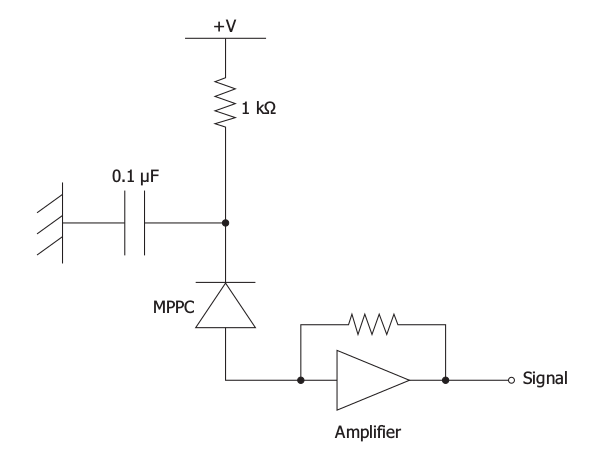
\includegraphics[scale=0.4]{CircuitoTarjeta.png}
\caption{\textbf{Figura 12}.- Circuito de una tarjeta tipo}
\end{figure}


Sabemos que utiliza un amplificador operacional... que nos ofrece una ganancia teórica de...  Para verificación de la misma se realizo un proceso de calibración. Para ello se introdujo una señal de....	similar a la señal emitida por un SiPM.



